\documentclass[usenames,dvipsnames,aspectratio=169]{beamer}
    \mode<presentation> {
    \usetheme{Montpellier}
    \useoutertheme{tree}
    \usecolortheme{beaver}
    %\setbeamertemplate{footline} % To remove the footer line in all slides uncomment this line
    \setbeamertemplate{footline}[page number] % To replace the footer line in all slides with a simple slide count uncomment this line
    \setbeamertemplate{navigation symbols}{} % To remove the navigation symbols from the bottom of all slides uncomment this line
    \setbeamersize{text margin left=8mm,text margin right=5mm}
    }

    \usepackage{graphicx} % Allows including images
    \usepackage{booktabs} % Allows the use of \toprule, \midrule and \bottomrule in tables
    \usepackage{minted}
    \usepackage{xcolor}
    \usepackage[utf8]{inputenc}
    \usepackage{pifont}
    \usepackage{xspace}
    \usepackage{newunicodechar}
    \usepackage{hyperref}

    \usepackage[pdf]{graphviz}

    \newunicodechar{✪}{\ding{74}}

    \definecolor{mintedbackground}{rgb}{0.95,0.95,0.95}
    \newcommand{\code}[1]{\colorbox{lightgray}{\texttt{#1}}}
    \newcommand{\distage}{\texttt{distage}\xspace}

\newminted{scala}{
    bgcolor=mintedbackground,
    fontfamily=tt,
    linenos=true,
    numberblanklines=true,
    numbersep=5pt,
    gobble=0,
    frame=leftline,
    framerule=0.4pt,
    framesep=2mm,
    funcnamehighlighting=true,
    tabsize=4,
    obeytabs=false,
    mathescape=false
    samepage=false, %with this setting you can force the list to appear on the same page
    showspaces=false,
    showtabs =false,
    texcl=false,
}

\newminted{text}{
    bgcolor=mintedbackground,
    fontfamily=tt,
    linenos=true,
    numberblanklines=true,
    numbersep=5pt,
    gobble=0,
    frame=leftline,
    framerule=0.4pt,
    framesep=2mm,
    funcnamehighlighting=true,
    tabsize=4,
    obeytabs=false,
    mathescape=false
    samepage=false, %with this setting you can force the list to appear on the same page
    showspaces=false,
    showtabs =false,
    texcl=false,
}

\newminted{json}{
    bgcolor=mintedbackground,
    fontfamily=tt,
    linenos=true,
    numberblanklines=true,
    numbersep=5pt,
    gobble=0,
    frame=leftline,
    framerule=0.4pt,
    framesep=2mm,
    funcnamehighlighting=true,
    tabsize=4,
    obeytabs=false,
    mathescape=false
    samepage=false, %with this setting you can force the list to appear on the same page
    showspaces=false,
    showtabs =false,
    texcl=false,
}

    \setminted{fontsize=\footnotesize,baselinestretch=1}

    \usepackage{tikz}
    \usetikzlibrary{positioning}
    \graphicspath{{target/media/}}

    \title{7mind: LSUG lightning talks}

    \institute[Septimal Mind Ltd]
    {
    Septimal Mind Ltd\\
    \medskip
    \textit{team@7mind.io}
    }
    \date{\today}


\makeatletter
\setbeamertemplate{headline}
{%
    \begin{beamercolorbox}[wd=\paperwidth,colsep=1.5pt]{upper separation line head}
    \end{beamercolorbox}
    \begin{beamercolorbox}[wd=\paperwidth,ht=2.5ex,dp=1.125ex,%
      leftskip=.3cm,rightskip=.3cm plus1fil]{title in head/foot}
      \usebeamerfont{title in head/foot}\insertshorttitle
    \end{beamercolorbox}
    \begin{beamercolorbox}[wd=\paperwidth,ht=2.5ex,dp=1.125ex,%
      leftskip=.3cm,rightskip=.3cm plus1fil]{section in head/foot}
      \usebeamerfont{section in head/foot}%
      \ifbeamer@tree@showhooks
        \setbox\beamer@tempbox=\hbox{\insertsectionhead}%
        \ifdim\wd\beamer@tempbox>1pt%
          \hskip2pt\raise1.9pt\hbox{\vrule width0.4pt height1.875ex\vrule width 5pt height0.4pt}%
          \hskip1pt%
        \fi%
      \else%
        \hskip6pt%
      \fi%
      \insertsectionhead
      \usebeamerfont{subsection in head/foot}%
      \ifbeamer@tree@showhooks
        \setbox\beamer@tempbox=\hbox{\insertsubsectionhead}%
        \ifdim\wd\beamer@tempbox>1pt%
          \ \raise1.9pt\hbox{\vrule width 5pt height0.4pt}%
          \hskip1pt%
        \fi%
      \else%
        \hskip12pt%
      \fi%
      \insertsubsectionhead\hfill\insertframenumber/\inserttotalframenumber\hspace{0.5em}
    \end{beamercolorbox}
    \begin{beamercolorbox}[wd=\paperwidth,colsep=1.5pt]{lower separation line head}
    \end{beamercolorbox}
}
\makeatother

  \begin{VerbatimOut}{ex-json-out.tmp}
{
"id": "john@doe.com",
"id.type": "email",
"balance":"42"
}
\end{VerbatimOut}


\begin{document}

\begin{frame}
%\titlepage

\begin{figure}
\color{RubineRed}
\Huge Zero-effort Structural Logging

\rule{\linewidth}{1mm}

\normalsize London Scala Users Group, Scala Community Day, 14/12/2019
\end{figure}

\begin{figure}
  Septimal Mind Ltd \\
  \textit{team@7mind.io} \\
  
\includegraphics[width=0.2\textwidth]{media/logo_7mind.png}
\end{figure}

\end{frame}

%%%%%%%%%%%%%%%%%%%%%%%%%%%%%%%%%%%%%%%%%%%%%%%%%%%%%%%%%%%%%%%%%%%%%%%%%%%%%%%%%%%%%%%%%%%%%%%%%%%
\section{Zero-effort structural logging}


\begin{frame}[fragile]
  \begin{figure}
  What would be the outcome of the following code?
  \end{figure}
\begin{scalacode}
val id = "john@doe.com"
val balance = 265
logger.info(s"User id=$id, balance=$balance")
\end{scalacode}
\end{frame}


\begin{frame}
  \begin{figure}
  \huge
  \texttt{User id=john@doe.com, balance=265}
  \end{figure}
\end{frame}


\begin{frame}[fragile]
  \begin{figure}
  There may be a bit different code as well:
  \end{figure}
\begin{scalacode}
val id = "+13023072835"
val balance = 42
logger.info(s"User id=$id, balance=$balance")
\end{scalacode}
\end{frame}

\begin{frame}
  \begin{figure}
  \huge
  \texttt{User id=+13023072835, balance=42}
  \end{figure}

  \begin{figure}
  \huge let's assume we've collected many logs and now we want 
  \end{figure}
\end{frame}

\begin{frame}
  \begin{figure}
  \huge let's assume we've collected many of these logs\dots \\
  \dots and we want to filter logs lines for users\dots \\
  \dots who registered with their email
  \end{figure}
\end{frame}

\begin{frame}
  \begin{figure}
  \large
  \texttt{grep -E -o "\b[A-Za-z0-9.\_\%+-]+@[A-Za-z0-9.-]+\.[A-Za-z]{2,6}\b" file.txt}
  \end{figure}

  \begin{figure}
  \Huge Oops\dots 
  \end{figure}
\end{frame}

\begin{frame}
  \begin{figure}
  \Huge Can we do it better?
  \end{figure}
\end{frame}

\begin{frame}[fragile]
  \begin{figure}
  \Huge We need structural logs
  \end{figure}


\begin{figure}
    \Large
    \inputminted{json}{ex-json-out.tmp}
\end{figure}
\end{frame}

\begin{frame}[fragile]
\begin{figure}
Almost all the structural logging libraries are very inconvenient\dots
\end{figure}
\begin{scalacode}
object Example {
  val LOG = FluentLoggerFactory
    .getLogger("fluentd.test")

  // ...

  val data =
      new HashMap[String, String]()
  data.put("id", userId)
  data.put("balance", userBalance.toString)
  LOG.log("user balance", data)
}
\end{scalacode}
\end{frame}

\begin{frame}[fragile]
\begin{figure}
But the code\dots
\end{figure}
\begin{scalacode}
val user = "JohnDoe"
logger.debug(s"Received a message from $user")
\end{scalacode}
\end{frame}

\begin{frame}[fragile]
\begin{figure}
\dots is always structured!
\end{figure}
\begin{scalacode}
Expr(Apply(Select(
  Apply(
    Select(Select(Ident("scala"), scala.StringContext),
      TermName("apply"))
      , List(Literal(Constant("Received a message from "))
          , Literal(Constant(""))
        )
  ),
  TermName("s")
  )
, List(Ident(TermName("user")))
))
\end{scalacode}
\end{frame}

\begin{frame}[fragile]
  \begin{figure}
  \Huge
  \color{RubineRed} L✪GSTAGE
  \noindent
  {\color{RubineRed} \rule{\linewidth}{1mm} }
  \Large First-class logging framework for Scala
  \end{figure}

  \begin{figure}
  \Huge So, we made a library \dots \\
  which can extract structure \dots 
  \end{figure}
\end{frame}

\begin{frame}
  \begin{figure}
  \large \dots so you may have text for humans
  \end{figure}

  \begin{figure}
    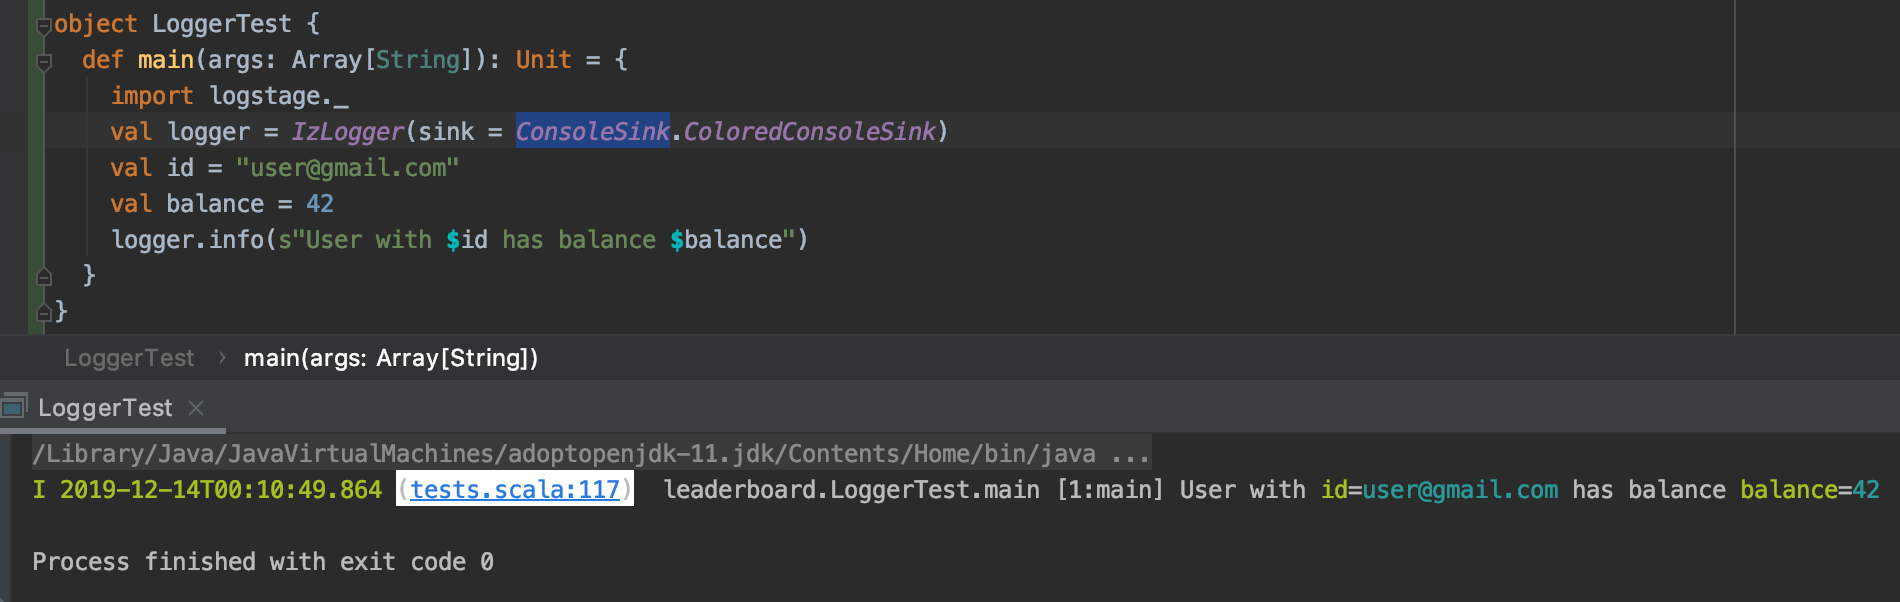
\includegraphics[width=0.95\textwidth]{media/text.png}
  \end{figure}
\end{frame}

\begin{frame}
  \begin{figure}
  \large \dots and nice JSON for robots
  \end{figure}

  \begin{figure}
    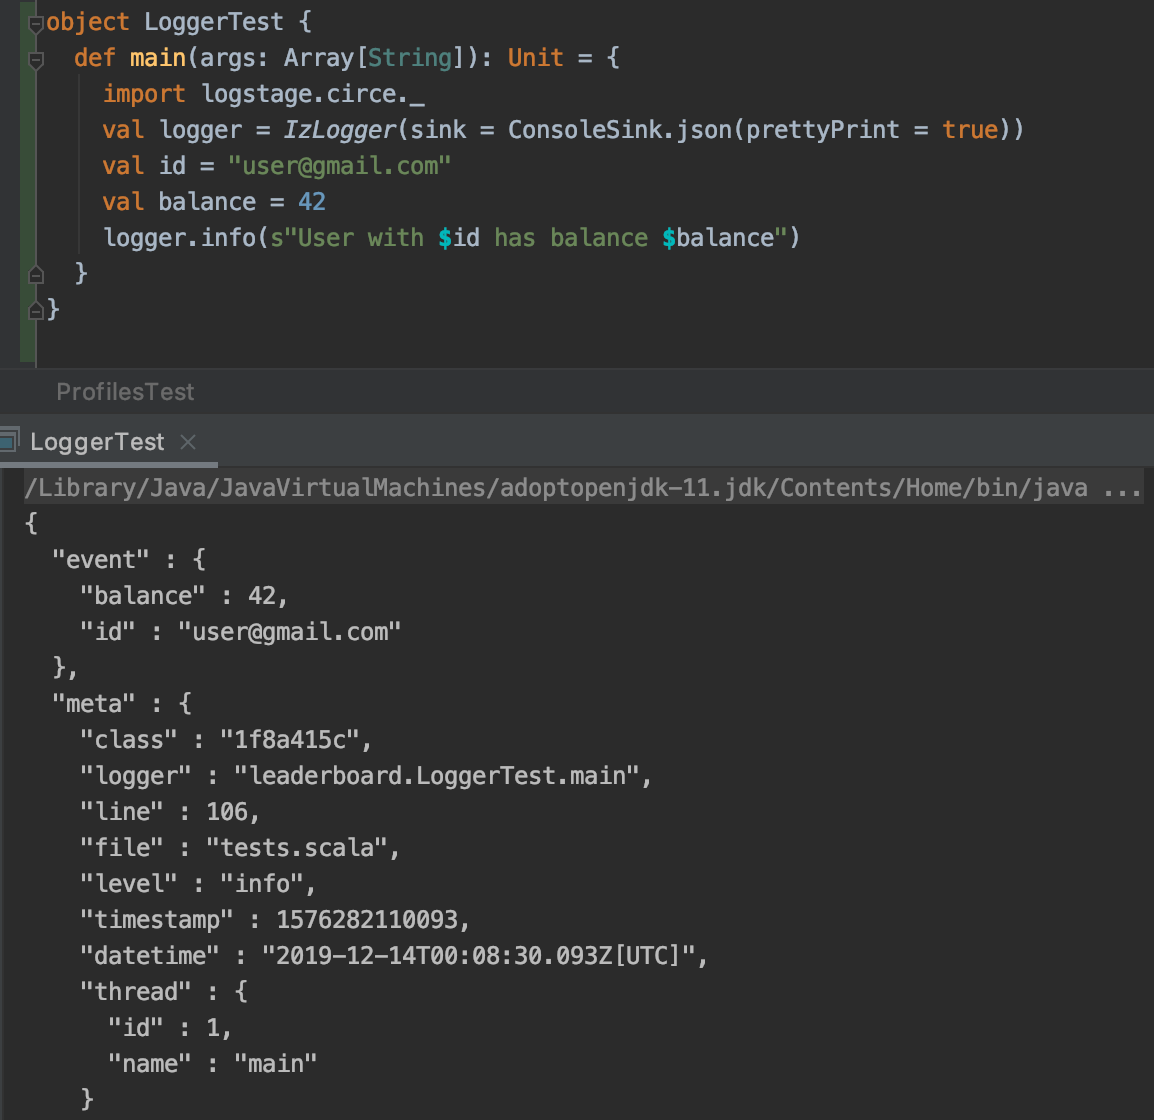
\includegraphics[width=0.55\textwidth]{media/json.png}
  \end{figure}
\end{frame}

\begin{frame}
  \begin{figure}
  \Huge Batteries included
  \end{figure}

  \begin{enumerate}
  \item \texttt{LogF[F[\_]]}
  \item \texttt{LogBIO[F[\_, \_]]}
  \item Better alternative for MDC
  \item \texttt{slf4j} adapter
  \item etc, etc\dots
  \end{enumerate}
\end{frame}


\begin{frame}
\begin{figure}
\color{RubineRed}
\Huge Dependency Injection for Scala done right

\rule{\linewidth}{1mm}

\normalsize London Scala Users Group, Scala Community Day, 14/12/2019
\end{figure}

\begin{figure}
  Septimal Mind Ltd \\
  \textit{team@7mind.io} \\
  
\includegraphics[width=0.2\textwidth]{media/logo_7mind.png}
\end{figure}
\end{frame}

\begin{frame}
  \begin{figure}
  \Huge Enigneers crave for good modularity\dots \\
  \large \dots There were at least 4 talks at FS2019 on this subject
  \end{figure}
\end{frame}

\begin{frame}
  \begin{figure}
  \Huge What we want from a good module system?
  \end{figure}

  \begin{enumerate}
  \item FP Support: ZIO envs, Effects, Resources\dots
  \item Speed
  \item Reliability: should fail fast, no reflection
  \item Transparency: introspections
  \item Scalability: should work for big apps
  \end{enumerate}
\end{frame}

\begin{frame}
  \begin{figure}
  \Huge What we have?
  \end{figure}

  \begin{enumerate}
  \item TF/implicits --- does not scale
  \item Cake pattern --- does not scale
  \item Guice, Spring? --- no, please!
  \item Airframe? --- no support for effects and resources
  \item Macwire? --- no support for effects and resources
  \end{enumerate}
\end{frame}

\begin{frame}
  \begin{figure}
  \Huge Are we out of options?
  \end{figure}
\end{frame}

\begin{frame}
  \begin{figure}
  \Huge \color{RubineRed} dist✪ge
  \end{figure}

  \begin{figure}
  \LARGE is a Dependency Injection mechanism for Scala
  \end{figure}

  \begin{figure}
  \large But it lacks negative traits of a typical DI thingy\dots \\
  \Large \dots and has many unique properties. \\
  \dots and it's blazing fast.
  \end{figure}

  \begin{figure}
  \large You may call it a module system for Scala\dots \\
  \Large \dots with automatic dependency-pruning solver
  \end{figure}
\end{frame}

\begin{frame}
  \begin{figure}
  \Huge What is Dependency Pruning in \distage?
  \end{figure}

  \begin{enumerate}
  \item Your application and tests may specify their dependencies semi-dynamically
  \item All the unnecessary components will not be even attempted to instantiate
  \item Technically it's very similar to Garbage Collection in JVM
  \end{enumerate} 
\end{frame}

\begin{frame}
  \begin{figure}
    \huge \distage performs optimal ahead of time planning.
    \\
    It doesn't  do any unnecessary job.
  \end{figure}
\end{frame}

\begin{frame}[fragile]
With \distage you can do this:

\begin{scalacode}
class JustATest[F[+_, +_]] {
  "service" must {
    "do something" in {
      (users: UserService[F], accounts: AccountingService[F]) =>
      for {
        user  <- users.create()
        balance <- accounts.getBalance(user)
      } yield {
        assert(balance == 0)
      }
    }
  }
}

object JustATestZioProd extends JustATest[zio.IO] with Prod
object JustATestZioDummy extends JustATest[zio.IO] with Dummy
\end{scalacode}
\end{frame}

\begin{frame}[fragile]
And this:

\begin{textcode}
laptop# docker run -ti company/product --run-all-services
prod01# docker run -ti company/product :analytics
prod02# docker run -ti company/product :accounting :users
\end{textcode}
\end{frame}

\begin{frame}
  \frametitle{Why it's a good idea to try \distage now}
  \begin{enumerate}
    \item Supports FP, wires Resources, Effects, ZIO Environments\dots
    \item Transparent and predictable
    \item Supports Roles and Dependency Pruning
      \begin{itemize}
        \item May \textbf{drastically} simplify development and operations workflows
        \item Helps you to write best tests possible without boilerplate
      \end{itemize}
    \item Promotes good practices and SOLID
    \item Most of the job is done in compile-time
    \item Safe
    \item Blazing fast
    \item no \texttt{scala-reflect} nor Java reflection, ScalaJS support is coming
    \item is non-invasive.
      \begin{itemize}
        \item You can add it to your project keeping business logic intact\dots
        \item \dots and remove it.
      \end{itemize}
    \item is not an ad-hoc thing, it has strong theory behind.
  \end{enumerate}
\end{frame}

\begin{frame}
  \begin{figure}
    \texttt{distage-framework} is the most productive way to write \\
    maintainable pure functional applications with ZIO. \\
    (And any other monad)
  \end{figure}
  \begin{figure}
    \texttt{distage-testkit} is the best way to make your tests performant and reliable.
  \end{figure}
  \begin{figure}
    \distage is adopted by several different companies and \\
    tested by two years of production usage.
  \end{figure}
\end{frame}


\begin{frame}
    \frametitle{Thank you for your attention}
    \begin{center}
      docs: \url{https://izumi.7mind.io}
    \end{center}
    \begin{center}
      \color{RubineRed}
      Septimal Mind is an Irish software consultancy and R\&D Company

      \vspace{0.3cm}
      We're looking for clients, contributors, adopters and colleagues ;)
    \end{center}
    \begin{center}
      Contact: team@7mind.io

      \vspace{0.3cm}
      Github: \url{https://github.com/7mind}

      \vspace{0.3cm}
      Slides: \url{https://github.com/7mind/slides}
    \end{center}
    \begin{center}
      \color{RoyalBlue}
      Follow us on Twitter

      \vspace{0.3cm}
      \url{https://twitter.com/shirshovp}

      \vspace{0.3cm}
      \url{https://twitter.com/kai_nyasha}
    \end{center}
\end{frame}

\end{document}
